\section{Vorlesung 14.10.2016}

\subsection{Grundlagen der Graphen und biologische Netze}
Graph: Knoten, Kanten (binäre Relationen)
\\\\
\underline{Transitivität:} implizite Verbindung (abhängig vom Kontext)

Labeled Graphs:
\begin{itemize}
	\item Graph: ($V$, $E$)
	\item Labels: L$_V$ (Knotenlabel), L$_E$ (Kantenlabel)
\end{itemize}

$e \in E \Rightarrow \exists \ x,y \in V:$ x und y sind die Endpunkte von e
\\\\
\underline{Knoten-Labelfunktion $\alpha$:} $\alpha:V \rightarrow L_V:v \mapsto \alpha(v)$\\
\underline{Kanten-Labelfunktion $\beta$:} $\beta:E \rightarrow L_E:e \mapsto \beta(e)$
\\\\
\textbf{ungerichtete Graphen}
\begin{itemize}
	\item Kante ist eine Menge von 2 (verschiedenen) Knoten
	\item $e = \{x,y\} = \{y,x\} \rightarrow$ Reihenfolge egal
	\item $E \subseteq V^{(2)} \rightarrow$ Kante ist Teilmenge von 2 Knoten
\end{itemize}

\textbf{gerichtete Graphen}
\begin{itemize}
	\item Kante ist ein geordnetes Paar von 2 (verschiedenen) Knoten
	\item $e = (x,y)$ entspricht $x \rightarrow y$, $(y,x)$ entspricht $y \rightarrow x$
	\item $E \subseteq V \times V$
	\item gerichtete Kante besteht aus head (in Pfeilrichtung) und tail
\end{itemize}

Funktionen gerichteter Graphen:\\
$h: E \rightarrow V: e \mapsto head(e)$\\
$t: E \rightarrow V: e \mapsto tail(e)$\\

Graphen in denen Kanten zwei verschiedenen Endpunkte haben \textbf{UND} zu jeden Paar von Knoten höchstens eine Kante gehört heißen \underline{EINFACH} oder \underline{SIMPLE}

im gerichteten Fall:\\
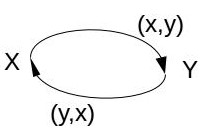
\includegraphics[width=0.25\textwidth]{lectures/161014/pix/1.jpg}
\\
trotzdem einfacher Graph!\\
\\
\underline{erst:}\\
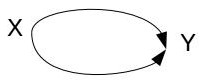
\includegraphics[width=0.25\textwidth]{lectures/161014/pix/2.jpg}
\\
ist Multigraph
\\\\
\textbf{Loops:}
\begin{figure}[ht]
	\centering
  	
\includegraphics[width=0.1\textwidth]{lectures/161014/pix/3.jpg}
  	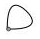
\includegraphics[width=0.1\textwidth]{lectures/161014/pix/4.jpg}
	\caption{links: gerichtet; rechts: ungerichtet}
\end{figure}

$\Rightarrow$ einfacher Graph mit Loops
\\\\
Durch Unterteilung der Kanten in Multigraphen kann eine Transformation in Graphen erzeugt werden:
\begin{itemize}
	\item ungerichtet: zweifache Unterteilung mittels zweier Knoten
	\item gerichtet: einfache Unterteilung mittels Knoten
\end{itemize}

\underline{vollständiger Graph:} jeder Knoten ist mit allen anderen Knoten verbunden $\rightarrow$ Anzahl Kanten=$\binom{n}{2}$

\subsection{Gleichheit von Graphen}
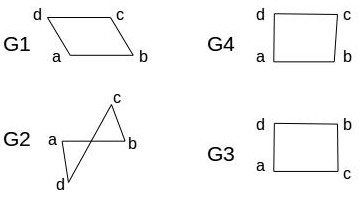
\includegraphics[width=0.5\textwidth]{lectures/161014/pix/5.jpg}\\
als labeled graphs: G$_1$=G$_2$=G$_4\neq$G$_3$\\\\
$\Rightarrow$ 2 Graphen G$_1$=(V$_1$, E$_1$) und G$_2$=(V$_2$, E$_2$) sind isomorph wenn es einen bijektive Abbildung\footnote{\url{https://de.wikipedia.org/wiki/Bijektive_Funktion}} $\pi:V_1 \rightarrow V_2$ gibt, sodass $\{x,y\} \in E_1 \Leftrightarrow \{\pi(x),\pi(y)\} \in E_2$
\\
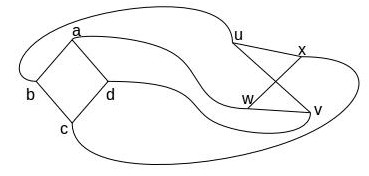
\includegraphics[width=0.5\textwidth]{lectures/161014/pix/6.jpg}
bijektive Abbildung: jedes Element von 1. wird zu genau einem Element von 2. zugeordnet\\\\
$\pi(a)=w, \pi(b)=u, \pi(c)=x, \pi(d)=v \\ \rightarrow$ hier ergibt bijektive Abbildung keinen Isomorpismus, da Bild(d) und Bild(c) Kante haben, jedoch v und x keine Kante haben\\\\
Durch folgende bijektive Abbildung wird aber Isomorphie erreicht:\\
$\pi(a)=w, \pi(b)=x, \pi(c)=u, \pi(d)=v$
\\\\
Bezogen auf die Labels kann es mehrere mögliche Isomorphien geben.
\\\\
Schreibweise: $G \simeq H$ (G ist isomorph zu H) mit 
$G\rightarrow^\pi H, G \leftarrow^{-\pi}H$ sodass $\pi$ isomorph ist
\\\\
\underline{Reflexivität:} Ein Graph ist zu sich selbst immer isomorph: $G \simeq G$\\
\underline{Symmetrie:} $G \simeq H \Leftrightarrow H \simeq G$\\
\underline{Transitivität:} $G \simeq H, H \simeq K \Rightarrow G \simeq K$\\
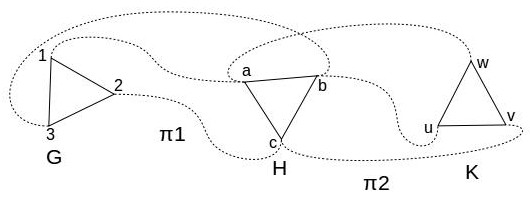
\includegraphics[width=0.75\textwidth]{lectures/161014/pix/7.jpg}
\\
$\simeq$ ist eine Äquivalenzrelation $\rightarrow$ Isomorphie teilt Graphen in Klassen ein (Isomorphieklassen)
\\\\
Nebenbemerkung: Labeled Graphen?\\
Zusätliche Bedingung benötigt: $\lambda(\pi(x))=\lambda(x) \rightarrow$ Labels müssen erhalten bleiben!
\\\\
\textbf{Testen auf Gleichheit}\\
Gegeben: G$_1$=(V$_1$, E$_1$), G$_2$=(V$_2$, E$_2$)\\
Frage: Sind die Graphen isomorph?
\newpage
Grundbedingungen:
\begin{enumerate}
	\item $|V_1| = |V_2| \rightarrow$ gleiche Anzahl von Knoten
	\item $|E_1| = |E_2| \rightarrow$ gleiche Anzahl von Kanten
\end{enumerate}

\subsection{Eigenschaften von Graphen}
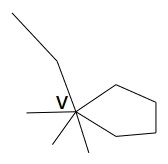
\includegraphics[width=0.25\textwidth]{lectures/161014/pix/8.jpg}\\
Nachbarknoten von v: $N(v):=\{y \in V|\{v,y\} \in E\}$\\
$deg(v):=|N(v)|$ … Anzahl der Nachbarknoten\\
$\delta(G):= \min \limits_{v \in V} deg(v)$ … Knoten aus G mit wenigstens Nachbarn\\
$\Delta(G):= \max \limits_{v \in V} deg(v)$ … Knoten aus G mit meisten Nachbarn\\
\\
\underline{Def:} Ein Graph heißt \textbf{REGULÄR} wenn $\Delta(G)=\delta(G)$\\(wenn alle Knoten gleichen Grad haben)
\\\\
\underline{Gradfolge von G:} aufsteigende Folge der Knotengrade aller Knoten eines Graphen\footnote{\url{https://de.wikipedia.org/wiki/Gradfolge}} $\mathcal{F}=(n_0,n_1,n_2,…,n_{|V|-1})$ mit $n_k:=|\{x \in V|deg(x)=k\}|$\\\\
$\delta(G) \geq 0$\\
$\Delta(G) \leq |V|-1$\\\\
Beispiel:\\
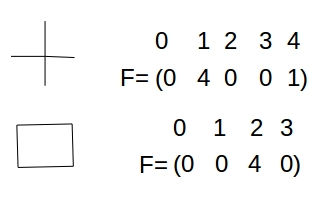
\includegraphics[width=0.5\textwidth]{lectures/161014/pix/9.jpg}\\
\\\\
\underline{bei Isomorphie:} $\mathcal{F}_1=\mathcal{F}_2 \rightarrow$ Isomorphismus $\pi$ erhält Grad der Knoten!

\subsection{Graph-Invarianten}
Eigenschaften, die unter Isomorphie erhalten bleiben\footnote{\url{https://en.wikipedia.org/wiki/Category:Graph_invariants}}\\
$\mathcal{G}$…Menge aller Graphen, F…ist ein Graphinvariant und X eine Eigenschaft wenn F: $\mathcal{G}$ $\rightarrow$ X die Eigenschaft hat, dass $G \simeq H \Rightarrow F(G) = F(H)$
\\\\
\underline{Invarianten bis jetzt:} $|V|, |E|,$ Gradfolge $\mathcal{F}$\\\\
Wenn F(G) $\neq$ F(H) für irgendeine Grapheninvariante $\Rightarrow$ G $\neg \simeq$ H

\subsection{Pfade und Zusammenhänge}

\underline{Kantenzug:} Folge von Kanten in G\\
$x_o,e_1,x_1,e_2,x_2,…,e_l,x_l$ sodass $e_i:=\{x_{i-1},x_i\}$\\\\
\underline{Beispiel:} (4,a,1,b,3,b,1,c,2)\\
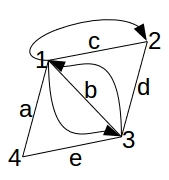
\includegraphics[width=0.25\textwidth]{lectures/161014/pix/10.jpg}\\
\underline{Weg:} Kantenzug sodass $e_i \neq e_j$ für $i \neq j$ (keine Kante doppelt verwenden)\\
Beispiel: (1,c,2,d,3,b,1,a,4,e,3))
\\\\
\underline{Pfad:} Kantenzug sodass $x_i \neq x_j$ für $(i,j) \neq (0,l)$ mit 0=Startknoten und l=Endknoten des Pfades (keinen Knoten mehrfach bis auf $x_0$, $x_l$)
\begin{itemize}
	\item offen: $x_o \neq x_e$ 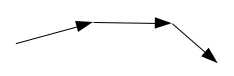
\includegraphics[width=0.2\textwidth]{lectures/161014/pix/11.jpg}
	\item geschlossen: $x_0=x_e$ (nur hier 1 Knoten doppelt benutzt!)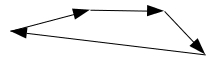
\includegraphics[width=0.2\textwidth]{lectures/161014/pix/12.jpg}
\end{itemize}

\fcolorbox{red}{white}{\parbox{\linewidth}{\underline{Definition:} G ist zusammenhängend wenn es zwischen je zwei Knoten x,y $\in$ V einen Kantenzug gibt}}
\\\\
\underline{Frage:}
\begin{enumerate}
	\item Ist Zusammenhang eine Grapheninvariante?
	\item Kann man in der Definition Kantenzug durch Weg, Pfad oder Kreis ersetzt?
\end{enumerate}